

\section{Making on-sky Sources%
  \label{making-on-sky-sources}%
}


\subsection{ScopeSim Templates%
  \label{scopesim-templates}%
}

An useful addition to the ScopeSim eco-system is the package \texttt{ScopeSim\_templates}.
This python package provides so-called helper functions for generating ScopeSim readable \texttt{Source} object for common astronomical objects.
The documentation for \href{https://scopesim-templates.readthedocs.io/en/latest/}{ScopeSim templates can be found on Read-The-Docs}

Here is a basic example of creating a star cluster using \texttt{ScopeSim\_templates}:

\phantomsection\label{code-scopesim-templates-example}
\begin{DUclass}{code}
\begin{DUclass}{plot}
\begin{quote}
\begin{alltt}
\begin{lstlisting}[frame=single]
from scopesim_templates.basic.stars import cluster

my_cluster = cluster(mass=1000, distance=50000, half_light_radius=1)
\end{lstlisting}
\end{alltt}
\end{quote}
\end{DUclass}
\end{DUclass}

% action: plot
% name: scopesim_templates_cluster_example
% ---
% plt.figure(figsize=(10,10))
% my_cluster.plot()
% plt.xlabel("x [arcsec]")
% plt.ylabel("y [arcsec]")

\begin{figure}[H]
\noindent\makebox[\linewidth][c]{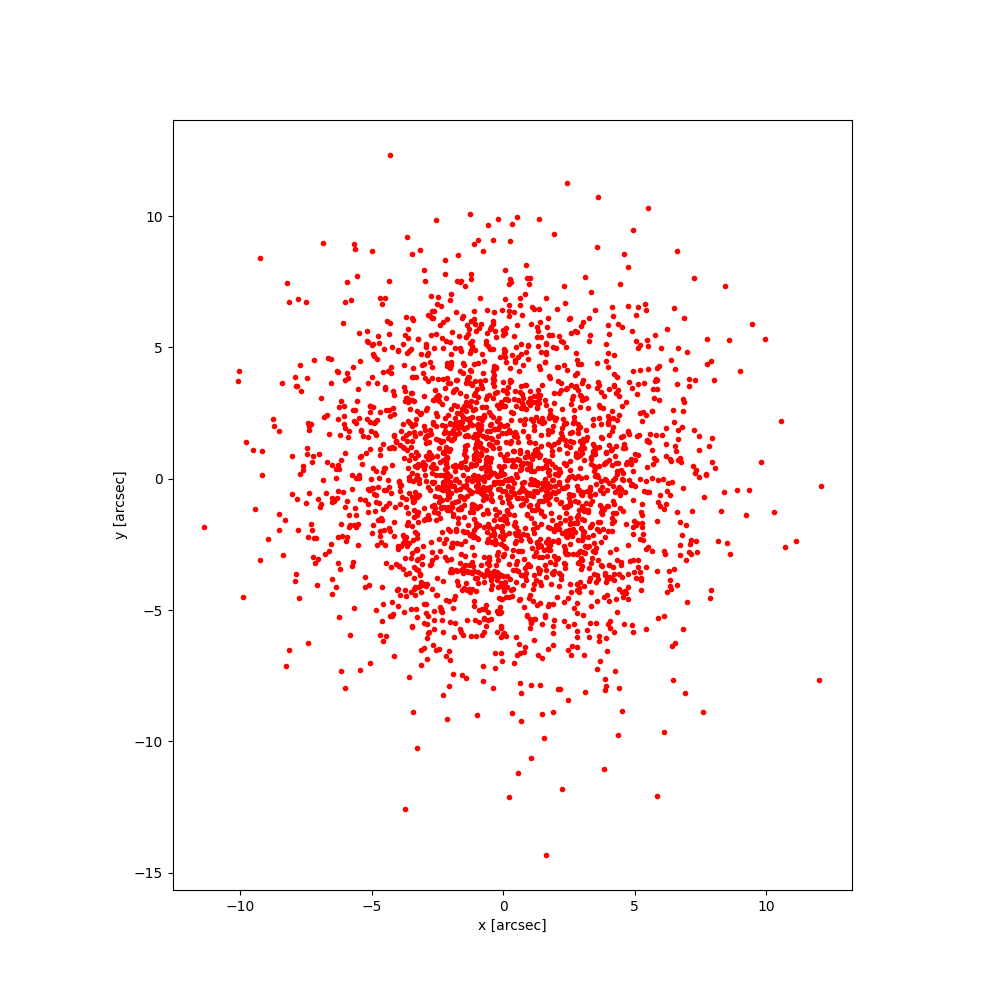
\includegraphics[scale=0.500000]{images/scopesim_templates_cluster_example.png}}\phantomsection\label{fig-scopesim-templates-cluster-example}

\caption{Left: the on-axis K-band (2.15$\mu$m) SCAO PSF for standrard atmospheric conditions.
Right: the K-band SCAO-PSF at the position (15, -5) arcseconds from the natural guide star.}
\end{figure}

\begin{itemize}
\item What is inside a Source object

\item 
\begin{description}
\item[{How to make source objects to observe}] \leavevmode 
\begin{itemize}
\item Star cluster

\item Custom point source

\item Elliptical galaxy

\item Custom extended source

\item Combining sources
\end{itemize}

\end{description}
\end{itemize}
